\documentclass[tikz,border=6pt]{standalone}
\usepackage{fontspec}
\usepackage{xeCJK}
\setmainfont{Times New Roman}
\setCJKmainfont{Hiragino Sans GB}
\setCJKsansfont{Microsoft YaHei}
\setCJKmonofont{STSong}
\usepackage{pgfplots}
\usepackage{xcolor}
\pgfplotsset{compat=1.18}

\definecolor{lineblue}{HTML}{4A90D9}
\definecolor{linered}{HTML}{E74C3C}

\begin{document}
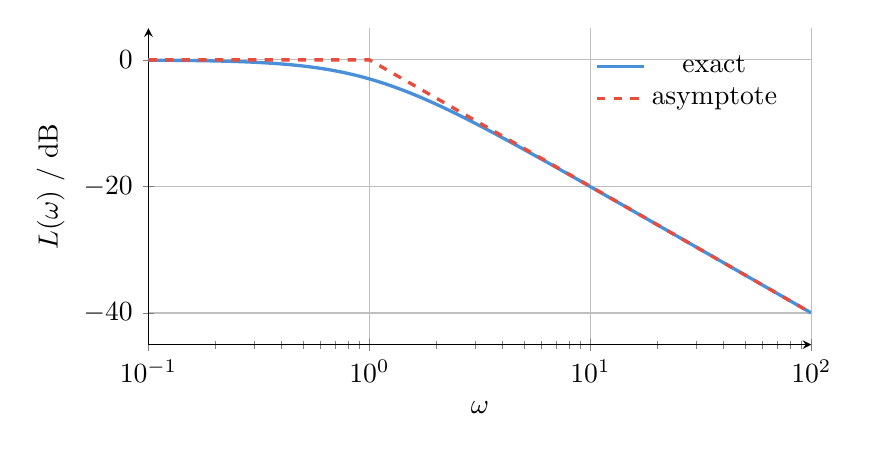
\begin{tikzpicture}
  \begin{axis}[
    width=10cm,
    height=5.6cm,
    xmode=log,
    xmin=0.1, xmax=100,
    ymin=-45, ymax=5,
    axis lines=left,
    xlabel={$\omega$},
    ylabel={$L(\omega)$ / dB},
    xtick={0.1,1,10,100},
    xticklabels={$10^{-1}$,$10^0$,$10^1$,$10^2$},
    ytick={-40,-20,0},
    grid=major,
    legend style={draw=none, fill=none, at={(0.97,0.95)}, anchor=north east}
  ]
    \addplot[lineblue, line width=1.2pt, domain=0.1:100, samples=200] {-10*ln(1+x^2)/ln(10)};
    \addlegendentry{exact}
    \addplot[linered, dashed, line width=1.2pt] coordinates {(0.1,0) (1,0) (100,-40)};
    \addlegendentry{asymptote}
  \end{axis}
\end{tikzpicture}
\end{document}
